\chapter{Enabling Structured Illumination Microscopy at greater depth}

\section{Sample Induced Aberrations in Thick Samples}
\label{sec:sample_aberrations_thick}

The origin of optical aberrations and their effect on image
formation from a geometric optics standpoint and how this leads 
decreased image quality and resolution has already been covered 
in Section~\ref{sec:aberrations}. The extent of optical 
aberrations in thick samples and the particular effects of
aberrations on structured illumination microscopy (SIM) imaging 
are worth paying particular attention to. 

In widefield microscopy, an even field of illumination is 
applied to the field of view and the resultant fluorescent
signal from the sample is measured. In SIM, this even 
illumination is replaced by a sinusoidally varying
illumination pattern. Multiple images with varying angle 
and phase shifts to the illumination pattern are acquired. 
These images are then used to reconstruct a single 
super-resolved image.\cite{gustafsson2000surpassing,gustafsson2008three}
Recall a single fluorescent image, $F(\bar{x})$, is 
defined by:

\begin{equation}\label{eq:SIM_fluorescent_image}
\begin{split}
	F(\bar{x}) &= (E \circledast H)(\bar{x})\\
	F(\bar{x}) &= [D(\bar{x})I(\bar{x})] \circledast H(\bar{x})\\
\end{split}
\end{equation}

Where $D(\bar{x})$ is the sample fluorescence distribution,
$I(\bar{x})$ is the illumination pattern, $E(\bar{x})$ is the 
resultant emission signal and $H(\bar{x})$ is the system point
spread function (PSF). Section~\ref{sec:aberrations} has already
discussed the effect aberrations have on distorting the system
PSF, $H(\bar{x})$. However, in SIM imaging the illumination 
pattern, $I(\bar{x})$, is also formed in the same imaging path
and is therefore the illumination pattern formation is also 
affected by the system aberrations.

Consider the illumination pattern function. Fully coherent
illumination conditions yeild optimum imaging performance and
are therefore chosen. In practice, only partially coherent 
conditions are achieveable. Utilising the fully coherent 
approximation, $I(\bar{x})$ can be expressed as:

\begin{equation}\label{eq:SIM_illumination}
	I(\bar{x}) = \left\| \frac{1}{2}[1 + \cos(\bar{x}\bullet\bar{p} + \phi)]\circledast H_{amp}(\bar{x}) \right\|^{2}
\end{equation}

Where $\bar{p}$ and $\phi$ define the orientation and phase of
the illumination pattern respectively. $H_{amp}(\bar{x})$ is the
amplitude PSF, as opposed to $H(\bar{x})$ which is the intensity
PSF and is defined as:

\begin{equation}\label{eq:amplitude_PSF}
	H_{amp}(\bar{x}) = \mathcal{F}[P(\bar{r})]
\end{equation}

Where $P$ is the pupil function, $\bar{r}$ is the coordinate
vector in the pupil plane and $\mathcal{F}$ is the Fourier
transform operation. Utiliting the Fourier convolution 
theorem, Equation~\ref{eq:SIM_illumination} becomes:

\begin{equation}\label{eq:SIM_illumination_invFT}
I(\bar{x}) = \left\| \mathcal{F}^{-1}\left\{\frac{1}{2}\left[\delta(\bar{r}) + \frac{\exp^{-i\theta}}{2}\delta(\bar{r}-\bar{p}) + \frac{\exp^{i\theta}}{2}\delta(\bar{r}+\bar{p})\right]P(\bar{r})\right\} \right\|^{2}
\end{equation}

Where value of $\bar{p}$ positions the delta functions in the
pupil plane. $\bar{p}$ is chosen to have a value of or close
to 1, to maximise the resolution increase. 
Equation~\ref{eq:SIM_illumination_invFT} there is clearly only
illumination at three points in the pupil plane, at the centre 
and diametrically opposed at the edge of the pupil. There are
two principle consequences of this fact. Firstly, since the 
illumination only exists at the centre and edges of the pupil
plane, the illumination pattern is only affected by phase 
variations at those points. Therefore, the illumination pattern
should be immune to aberrations with little phase variation at 
the edges of the pupil. Secondly, rotationally symmetrical 
aberrations, such as spherical aberration, have have the main
effect of refocusing the illumination pattern.\cite{booth2015aberrations}

It has also been shown that the imaging properties of a SIM
system and the quality of the reconstructed super-resolution
images is determined by the system's ability to reliably
image the high spatial frequencies.\cite{debarre2008adaptive,thomas2015enhanced}
The aberrations which affect the strength of high spatial 
frequency signals can be divided into two categories; 
isoplanar and anisoplanar aberrations. Single adaptive 
elements, such as the deformable mirror in the DeepSIM 
setup, can only correct for the isoplanar aberrations.
Anisoplanar aberrations will still introduce artifacts 
in the final, resonstructed data. However, provided that
the anisoplanar aberrations are considerably smaller than
the isoplanar aberrations, these aberrations will be small
compared to the SIM image and will not prevent a successful
reconstruction.\cite{thomas2015enhanced}

The cummulative effects of the optical aberrations is that
traditional SIM imaging is limited in its imaging depth to
approximately $10-20\mu m$.\cite{schermelleh2019super,wu2018faster} However, 
correcting the optical aberrations present would not yeild
an infinite depth of imaging due to scattering of photons,
which increases with depth. Nonetheless, by correcting for
optical aberrations present DeepSIM offers the potential to 
acquire super-resolution SIM images at an unprecidented depth.

\section{IsoSense}
\label{sec:isosense}

Anisotropies in the sample fluorescence distribution can bias 
the corrections towards improving the image quality in a 
non-uniform manner. There has recently been a technique developed 
to overcome  this issue; IsoSense\cite{vzurauskas2019isosense}. 
It relies  on producing spatially structured light in order to fill 
empty sections of the image Fourier spectrum. IsoSense is designed 
to be used in structured illumination microscopy (SIM) setups since 
they often incorporate spatial light modulators (SLM) as high-speed, 
dynamic diffraction  gratings and SIM is particularly sensitive to 
Fourier space anisotropies.

Microscope-AOtools incorporates the methods necessary to implement
IsoSense. Figure~\ref{fig:isosense_visualisation} shows both
the structured illumination pattern applied to the SLM 
and the location of the beams in Fourier space. The illumination
pattern shown in Figure~\ref{fig:isosense_visualisation_real} is
the inverse Fourier transform of the 4-beam interference pattern 
in Figure~\ref{fig:isosense_visualisation_ft}. The location 
of these beams, $\bar{\kappa}$, are: 
$(0,0)$, $(0,\gamma w)$, $(0,-\gamma w)$, $(\gamma w, 0)$, 
$(-\gamma w, 0)$, $(\frac{\gamma w}{2}, \frac{\gamma w}{2})$, 
$(-\frac{\gamma w}{2}, \frac{\gamma w}{2})$, $(\frac{\gamma w}{2},
-\frac{\gamma w}{2})$, $(-\frac{\gamma w}{2}, 
-\frac{\gamma w}{2})$. $u,v$ are the spatial frequency 
analogues of the $x,y$ axes. $w$ is the Abbe diffraction limit and 
$\gamma$ is a user defined fill fraction. This fill
fraction controls the positions of the beams in the interference
pattern and hence the region of the Fourier spectrum which will 
be enhanced over normal illumination. The resultant emission image 
obtained, $E(\bar{x})$, can be described as:

\begin{equation}\label{eq:isosense_real}
E(\bar{x}) = D(\bar{x}) \times I(\bar{x})
\end{equation}	

Where $I(\bar{x})$ is the interference pattern, similar to that shown in 
Figure\ref{fig:isosense_visualisation_real}, $D(\bar{x})$ is the sample 
fluorescence distribution as before and $\bar{x}$ is the spatial 
coordinate vector. Applying a Fourier transform yields:

\begin{equation}\label{eq:isosense_ft}
\begin{split}
\mathcal{F}[F(\bar{x})] &= \mathcal{F}[D(\bar{x})\times I(\bar{x})] \\
\tilde{\textbf{F}}(\bar{k}) &= \tilde{\textbf{D}}(\bar{k}) \circledast \tilde{\textbf{I}}(\bar{k}) \\
\tilde{\textbf{F}}(\bar{k}) &= \sum_{\bar{\kappa}}\iint\tilde{\textbf{D}}(\bar{k})\delta(\bar{k} - \bar{\kappa})dudv \\
\tilde{\textbf{F}}(\bar{k}) &= \sum_{\bar{\kappa}}\tilde{\textbf{D}}(\bar{k} - \bar{\kappa})
\end{split}
\end{equation}

Where $\tilde{\textbf{F}}(\bar{k})$, $\tilde{\textbf{I}}(\bar{k})$ and 
$\tilde{\textbf{D}}(\bar{k})$ are the Fourier transforms of $F(\bar{x})$, 
$I(\bar{x})$ and $D(\bar{x})$, the $\bar{\kappa}$ frequencies are the 
locations of interference pattern beams described above and $\bar{k}$ is 
the spatial frequency vector. By convolving the sample fluorescence 
distribution with  multiple $\delta$-functions, multiple copies of the 
sample spatial frequency information are created and regions of the 
system OTF left  unfilled by sample fluorescence distribution anisotropies 
are filled, leading to  improved sampling of the system OTF particularly 
at high spatial frequencies close to $w$ and greater aberration 
sensitivity.\cite{vzurauskas2019isosense}

\begin{figure}[h]
	\centering
	\begin{subfigure}{0.4\textwidth}
		\centering
		
\includegraphics[width=1\linewidth, scale=0.5]{./images/isosense_visualisation_real.png}
		\caption{}
		\label{fig:isosense_visualisation_real}
	\end{subfigure}
	\begin{subfigure}{0.4\textwidth}
		\centering
		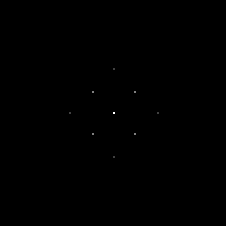
\includegraphics[width=1\linewidth, scale=0.5]{./images/isosense_visualisation_ft.png}
		\caption{}
		\label{fig:isosense_visualisation_ft}
	\end{subfigure}
	\caption{(a) A simulated IsoSense pattern created with a 4-beam interference. A pattern similar to this is applied to the SLM (b) A diagram of a 4 beam interference pattern in Fourier space. The diagonal axis and the horizontal/vertical axis have $\frac{1}{2}$ and $\frac{1}{4}$ of the intensity of the central beam respectively.}
	\label{fig:isosense_visualisation}
\end{figure}

\section{Biological Exemplar}
\label{sec:SIM_biology}

\begin{itemize}
	\item Explain why the particular sample needs the correction provided, what you can't normally resolve without AO and show how  AO improves it.
\end{itemize}

\subsection{Experimental Setup}
\label{subsec:SIM_setup}

\subsection{Sample preparation}
\label{subsec:SIM_sample_prep}

\section{Experimental Results}
\label{sec:SIM_results}
